%\documentclass[../../tesis.tex]{subfiles}
\documentclass[class=article, crop=false]{standalone}
\usepackage[subpreambles=true]{standalone}
\usepackage{import}
\graphicspath{{images/}}


%
%
%
%
\usepackage{amssymb}
\usepackage{amsmath}
%\usepackage{natbib}
\setcounter{tocdepth}{3}
\usepackage{graphicx}
%\graphicspath{ {Graficos/} }
\usepackage{subfigure}
\usepackage{gensymb}
\usepackage{authblk}
\usepackage{url}
\usepackage[utf8]{inputenc}

\usepackage[spanish]{babel}
\selectlanguage{spanish}
%\usepackage[style=authoryear]{biblatex}
\begin{document}
	
\subsubsection{Definiciones}

\begin{itemize}
\item
Un \textbf{\emph{producto}} es la \emph{unidad básica discreta de los
	datos}, se define como un ítem de un nomenclador (SITC). Se representa
como un vector unitario. Definimos el superíndice \(i\) del vector
como el i-ésimo producto del nomenclador y el i-ésimo elemento del
vector. El V-ésimo producto del nomenclador es el vector \(w\), tal
que \(w^v\)=1 y \(w^u\)=0, \(u\neq v\)
\item
Un \textbf{\emph{país}} es una secuencia de \textbf{N} productos,
definido como \(W= (w_1, w_2, ..., w_N)\)
\item
Nuestro \textbf{corpus} es la colección de \textbf{M} países, definido
como \(D = (d_1, d_2,..., d_M)\)
\item
Un \textbf{\emph{componente}} es una dimensión latente sobre el
corpus, y suponemos una cantidad fija \emph{k} de los mismos.
\item
Nuestro objetivo es obtener:
\end{itemize}

\begin{enumerate}
\def\labelenumi{\arabic{enumi}.}
\item
Una distribución de componentes sobre cada país.
\item
Una distribución de los productos sobre los componentes.
\end{enumerate}


\subsubsection{Dimensión latente}

\begin{figure}
\centering
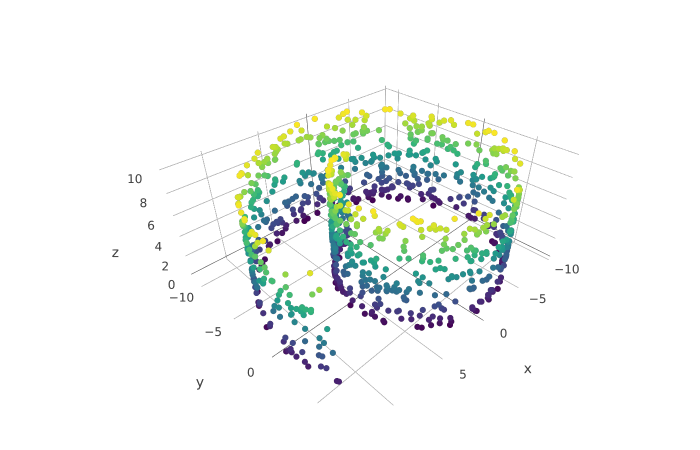
\includegraphics[width=0.5\textwidth]{swissRoll.png}
\caption{Swiss Roll}
\end{figure}

\begin{itemize}
\item
Nuestros datos están definidos en una dimensión alta
\[\mathcal{R}^{N*P*Y*T}\]
\item
Podemos encontrar un espacio de menor dimensión en el que se logra
representarlos bien
\end{itemize}

\subsubsection{Proceso generativo}

Intuitivamente, suponemos el siguiente proceso generativo de datos:

\begin{itemize}
\item
Para cada país del corpus, imaginamos que las exportaciones surgen de
un proceso de dos etapas:

\begin{itemize}
	\item
	Elegimos aleatoriamente una distribución sobre los componentes
	\item
	Para cada dólar exportado:
	
	\begin{itemize}
		\item
		Elegimos aleatoriamente el componente al que pertence, dada la
		distribución definida en el paso anterior
		\item
		Elegimos aleatoriamente un producto de la distribución
		correspondiente a dicho componente
	\end{itemize}
\end{itemize}
\end{itemize}

\begin{enumerate}
\def\labelenumi{\arabic{enumi}.}
\item
Para cada Componente \(k \in \{1,2,... K\}\)
\end{enumerate}

\begin{itemize}
\item
Generar una distribución sobre los componentes
\(\beta \sim Dir_v(\eta)\) con \(\eta \in \mathcal{R_{>0}}\) un
parámetro fijo
\end{itemize}

\begin{enumerate}
\def\labelenumi{\arabic{enumi}.}
\setcounter{enumi}{1}
\item
Para cada país \(d \in \{1,2,... D\}\)
\end{enumerate}

\begin{itemize}
\item
generar un vector de proporciones de componentes
\(\theta_d \sim Dir_K(\alpha)\) con \(\alpha \in \mathcal{R_{>0}^K}\)
un parámetro fijo
\item
Para cada dólar exportado:

\begin{enumerate}
	\def\labelenumi{\roman{enumi}.}
	\item
	generar una asignación del componente \(z_{dn} \sim Mult(\theta_d)\)
	\item
	asignar el producto \(w_{dn} \sim Mult(\beta_{zn})\)
\end{enumerate}
\end{itemize}


\subsubsection{Representación gráfica}

\begin{figure}
\centering
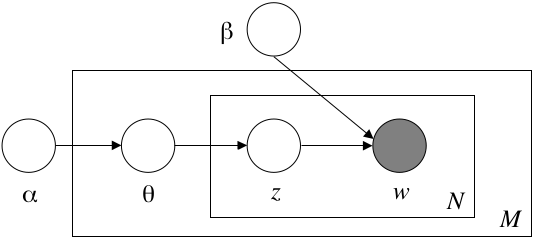
\includegraphics[width=0.5\textwidth]{grafo.png}
\caption{\cite{blei2003latent}}
\end{figure}

\begin{itemize}
\item
Cada nodo representa una distribución de probabilidad.
\item
La arista significa que la distribución de salida define los
parámetros de la distribución de entrada
\item
Los recuadros significan replicación:

\begin{itemize}
	\item
	El recuadro interior representa que el proceso se realiza para cada
	dólar exportado en el país.
	\item
	El recuadro exterior representa que el proceso se realiza para cada
	país en el corpus.
\end{itemize}
\end{itemize}

\subsubsection{Distribución de Dirichlet}

Un Proceso de Dirichlet es una familia de procesos estocásticos donde
\textbf{las realizaciones son ellas mismas distribuciones de
probabilidad.}

Es decir, el rango de esta distribución (así como en una normal son los
reales) son distribuciones de probabilidad.

\begin{figure}
\centering
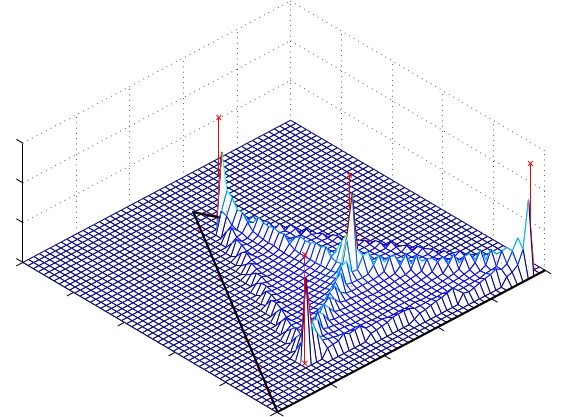
\includegraphics[width=0.5\textwidth]{dirichlet.png}
\caption{\cite{blei2003latent}}
\end{figure}

Para interpretarlo geométricamente, podemos pensar un ejemplo de la
distribución de densidad para \textbf{3 productos} y \textbf{4
componentes}.

\begin{itemize}
\item
El triángulo representa todas las distribuciones (multinomiales)
posibles sobre los tres productos
\item
Cada uno de los vértices del triángulo es una distribución de
probabilidad que asigna una probabilidad de 1 a uno de los productos.
\item
El punto medio de cada lado, es una distribución con probabilidad 0.5
a dos componentes.
\item
El cuarto componente, el centroide del triángulo, asigna probabilidad
de \(\frac{1}{3}\) a cada producto.
\item
Los cuatro puntos marcado con x son las distribuciones multinomiales
de p(w\textbar{}z) para cada uno de los cuatro componentes.
\item
La altura en el eje z es una posible distribución de densidad sobre el
simplex, es decir, sobre las distribuciones de densidad multinomiales,
dada por LDA
\end{itemize}

\subsubsection{Inferencia}

Cuando observamos los datos, no contamos con los tópicos ni con su
distribución, sino con los productos y países. El objetivo es realizar
inferencia sobre las variables latentes, mediante el Teorema de Bayes:

\[
p(\theta,z|w,\alpha,\beta) = \frac{p(\theta,z,w|\alpha,\beta)}{p(w|\alpha,\beta)}
\]

Nuestra función objetivo es:

\[
\ell(\alpha, \beta) = \sum_{d=1}^M \log p(w_d|\alpha,\beta)
\]

El problema es que esta ecuación es intratable, por la interacción entre
\(\theta\) y \(\beta\)

Por ello, la inferencia se realiza sobre una familia de modelos que se
sabe que son una cota inferior de probabilidad, y que son tratables.

\begin{itemize}
\item
Estos modelos tienen parámetros variacionales, que se ajustan para
obtener el modelo que más se acerca a la cota inferior.
\item
La forma de obtener una familia de modelos tratables es considerar
algunas modificaciones sobre el modelo gráfico original, removiendo
nodos y aristas.
\end{itemize}

\begin{figure}
\centering
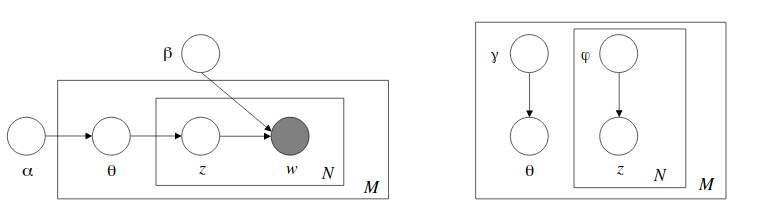
\includegraphics[width=0.65\textwidth]{grafo_variational.png}
\caption{\cite{blei2003latent}}
\end{figure}

\subsubsection{Estimación de parámetros}

Podemos aproximar los parámetros alternando el proceso de
\emph{variational Expectation Maximization} (EM):

\begin{itemize}
\item
\textbf{paso E}: Optimizamos los parámetros variacionales
\(\gamma, \varphi\)
\item
\textbf{paso M}: Para los valores fijos \(\gamma, \varphi\),
maximizamos la cota inferior respecto a los parámetros del modelo,
\(\alpha,\beta\)
\end{itemize}

Estos dos pasos se alternan hasta converger.

Por último, se realiza un suavizado sobre las probabilidades que un
componente asigna a un producto, para que sean siempre mayores a 0.






%\bibliographystyle{unsrt}
%\bibliography{bibliografia}
%
\end{document}

